\subsection{Die Americium-Quelle}

Am241 ist ein $\alpha$-Strahler. Das heißt, es werden Helium-Kerne bestehend aus zwei Protonen und zwei Neutronen emittiert,
die in diesem Versuch anschließend auf eine Goldfolie treffen. Das Zerfallsschema ist in Abbildung \ref{fig:zerfall} zu sehen.
Das Americiumatom zerfällt also in ein $\alpha$-Teilchen und in ein Np237-Atom.

\begin{center}
  $^{95}_{241}$Am \rightarrow $^{93}_{237}$Np + $^{2}_{4}$He
\end{center}

Aufgrund des Massendefekts wird beim Zerfall Energie frei, die sich als kinetische Energie der beiden Zerfallsprodukte
manifestiert. Das Americium kann direkt in den Grundzustand des Np237 zerfallen (was jedoch sehr unwahrscheinlich ist, siehe Abbildung
\ref{fig:zerfall}) oder zunächst in einen angeregten Zustand. Durch das Emittieren von Photonen kann dann der Grundzustand
erreicht werden.

\begin{figure}
\centering
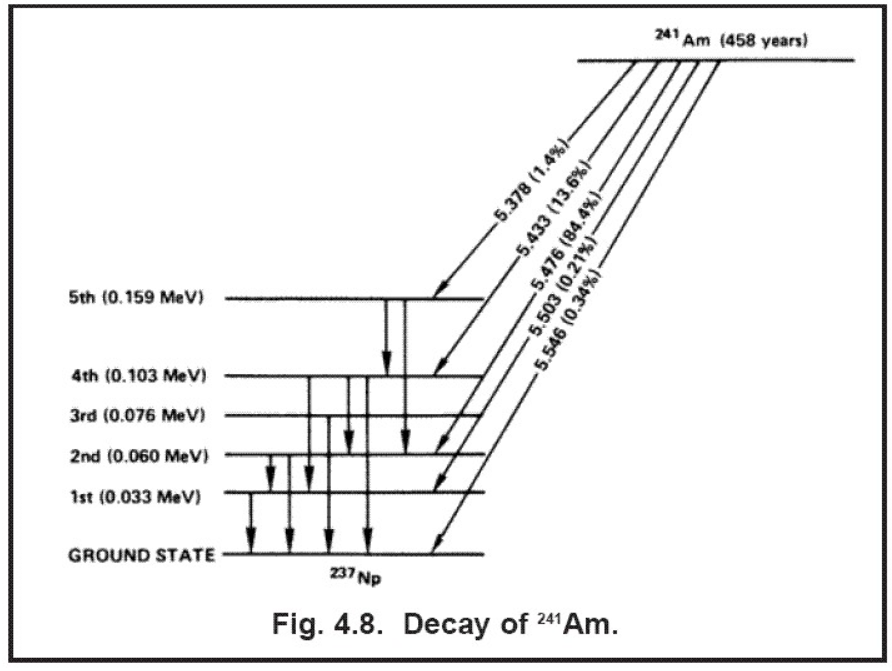
\includegraphics[width=0.7\textwidth]{zerfall.png}
\caption{Zerfallsschema von Am241 \cite{gsi}.}
\label{fig:zerfall}
\end{figure}

\subsection{Wechselwirkung in Materie}

Geladene Teilchen wie die $\alpha$-Teilchen wechselwirken in einem Medium mit den Atomen in diesem Medium. Da $\alpha$-Teilchen
eine große Masse und elektrische Ladung besitzen, wechselwirken sie stark mit den Atomen in ihrer Umgebung, sodass ihre
Reichweite stark begrenzt ist. Des Weiteren hängt ihre Reichweite von der Dichte des Materials ab.
Ein dickeres Blatt Papier oder ein Abstand von wenigen Zentimetern zur Strahlungsquelle reicht somit schon aus, um sich vor der
$\alpha$-Strahlung zu schützen.

Eine Wechselwirkung kann zum Beispiel durch Anregung der Atome im Material stattfinden. Eine andere Möglichkeit liegt darin,
dass ein $\alpha$-Teilchen ein Atom ionisiert. Die Strahlung verliert dabei an Energie und die Teilchen erfahren eine
Richtungsänderung.

\begin{figure}
\centering
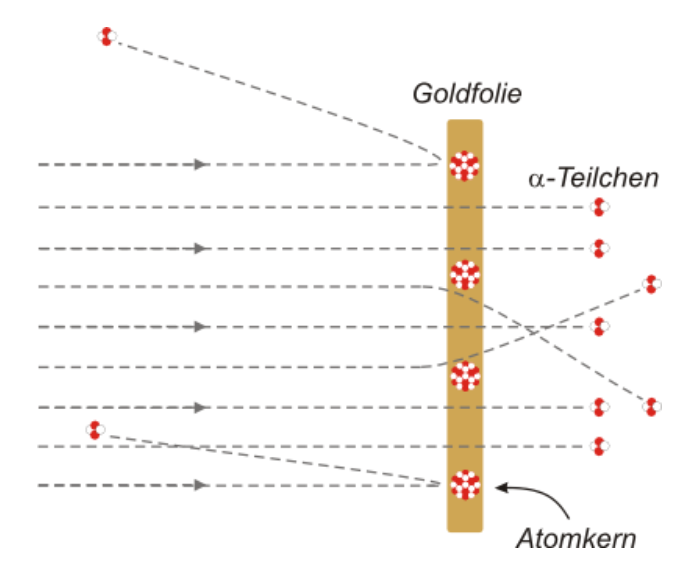
\includegraphics[width=0.7\textwidth]{rutherfordschema.png}
\caption{Schema zum Rutherfordversuch \cite{unigoett}.}
\label{fig:streu}
\end{figure}

Der Energieverlust pro Weglänge kann durch die Bethe-Bloch-Formel berechnet werden. Sie gilt jedoch nur für niedrige
Energien.

\begin{equation}
\frac{\mathrm{d}E}{\mathrm{d}x}=\frac{4\pi e^4z^2n Z}{m_ev^2(4\pi\epsilon_0)^2}\log{\left(\frac{2m_ev^2}{I}\right)}
\end{equation}

Dabei ist $Z$ die Ladungszahl des Mediums, $n$ die Anzahl der Atome pro $m^3$, $I=Z*10$eV die mittlere Ionisationsenergie,
$z$ die Ladungszahl der $\alpha$-Teilchen und $m_{\alpha}$ die Masse der $\alpha$-Teilchen. $v$ ist ihre Geschwindigkeit.

Somit beträgt beispielsweise das Bremsvermögen der Teilchen in Luft (genähert als reines Stickstoff)

\begin{equation}
\frac{dE}{dx}=\SI{0,4}{\mega\electronvolt} .
\end{equation}

Die Bethe-Bloch-Formel kann außerdem so umgeformt werden, dass die Reichweite d$x$ bestimmt werden kann:

\begin{equation}
dx = dE\frac{4\pi m_e v^2\epsilon^2_0}{e^4z^2nZ}\log^{-1}\left(\frac{2m_e v^2}{I}\right) .
\end{equation}

\subsection{Der Wirkungsquerschnitt}

Der Wirkungsquerschnitt ist ein Maß für die Wahrscheinlichkeit, dass zwei Teilchen miteinander wechselwirken. Der differentielle
Wirkungsquerschnitt beschreibt dabei die Intensitätsverteilung über alle Raumrichtungen $\Omega$.

Mit Hilfe der Rutherfordschen Streuformel kann die Wahrscheinlichkeit berechnet werden, dass ein gestreutes Teilchen nach der
Ablenkung um einen Winkel $\theta$ im Raumwinkel d$\Omega$ auftritt.

\begin{equation}
\frac{\mathrm{d}\sigma}{\mathrm{d}\Omega}(\theta)=\frac{1}{(4\pi\epsilon)^2}\left(\frac{z Z e^2}{4 E_{\alpha}}\right)^2\frac{1}{\sin^4{\left(\frac{\theta}{2}\right)}}
\end{equation}

Diese Formel gilt jedoch nur unter der Annahme, dass keine Mehrfachstreuung stattfindet. Die Folie im Experiment sollte
also möglichst dünn sein. Außerdem wird angenommen, dass nur die Coulombwechselwirkung wirkt. Kernkräfte werden vernachlässigt.
Des Weiteren sollte die Masse des Targets deutlich größer als die des Projektilteilchens sein.

($E_{\alpha}$: mittlere Energie der $\alpha$-Teilchen, $z$: Ladungszahl des gestreuten Teilchens, $Z$: Ladungszahl des Atomkerns)

Der Gesamtwirkungsquerschnitt lautet dann

\begin{equation}
  \sigma = \int \frac{\mathrm{d}\sigma}{\mathrm{d}\Omega}\mathrm{d}\Omega .
\end{equation}
